Getblocktemplate, or GBT, was born over the \textbf{mid 2012}. 
It was the first alternative to the \textit{getwork} method, openly developed by some of the most skilled Bitcoin Core developers of that time, promoted and directed firstly by the Bitcoin Core developer Luke Dashjr. The official announcement of GBT was made by Luke Dashjr himself on 12th September 2012, on Bitcoin Talk Forum \cite{bitcointalkDecentralizedMining}.
\begin{figure}[h!]
    \centering
    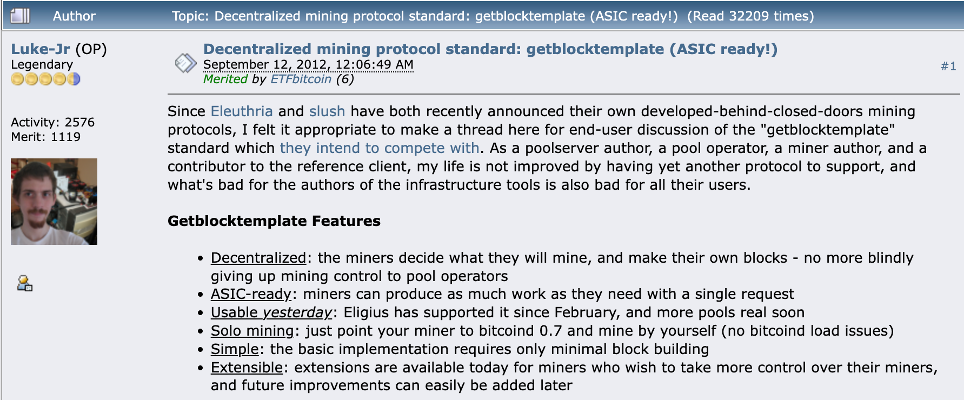
\includegraphics[width=15cm]{Figures/gbt/gbt1.png}
    \caption{Luke-Jr \textit{getblocktemplate}  announcement, Bitcoin Talk Forum}
    \label{fig:gbt1}
\end{figure}
\newline
\noindent GBT was defined as a new mining protocol standard, developed to accommodate both solo mining and pooled one, thanks to its usage flexibility. 
The main reason why it was developed was the need to find a solution for the issue described at the end of the previous chapter: miners were becoming more and more powerful, and the nonce research space of the previous getwork method was not enough for the maximum hashrate of the newest equipment. \\
Getblocktemplate introduced different new features to the mining operations of that time, but the most important point which mainly drove the entire development (apart from the solution at the nonce research space issue) was the attempt to decentralize the power obtained from the mining pool operators. At that time, as said in the previous chapter, most of the miners were using the getwork method in a pooled mining context: in this way the only entities responsible for building the blocks, selecting the transactions from the mempool, were the pools themselves. Most miners were just mining onto the block headers received from the pool server, never building their own block templates: this was a huge security risk from the point of view of the GBT developers and supporters, that could have led to a high single-point failure and censorship risk. \\\\
The group of developers involved into GBT followed the standard procedure for proposing and implementing new features into Bitcoin Core: they published two Bitcoin Improvement Proposal(s) \cite{cointelegraphWhatBitcoin}, specifically BIP22 and BIP23.\\
Getblocktemplate was officially implemented in Bitcoin Core release v.0.7.0, on 17th September 2012 \cite{bitcoinBitcoinQtVersion}.

